% Classic priority inversion — three-task timeline
% tau_H (high), tau_M (medium), tau_L (low).
% tau_L holds mutex R; tau_H blocks on R; tau_M preempts tau_L -> inversion.
% Right panel shows PIP fix: tau_L inherits tau_H priority, blocks tau_M.
\documentclass[border=5pt]{standalone}
\usepackage{lmodern}
\usepackage{tikz}
\usetikzlibrary{arrows.meta,patterns,decorations.pathreplacing}

\definecolor{kmblue}{HTML}{003874}
\definecolor{kmgold}{HTML}{BA9224}
\definecolor{rtgreen}{HTML}{1F9D55}
\definecolor{rtred}{HTML}{E3342F}
\definecolor{axgray}{HTML}{888888}
\definecolor{dkgray}{HTML}{555555}

\begin{document}
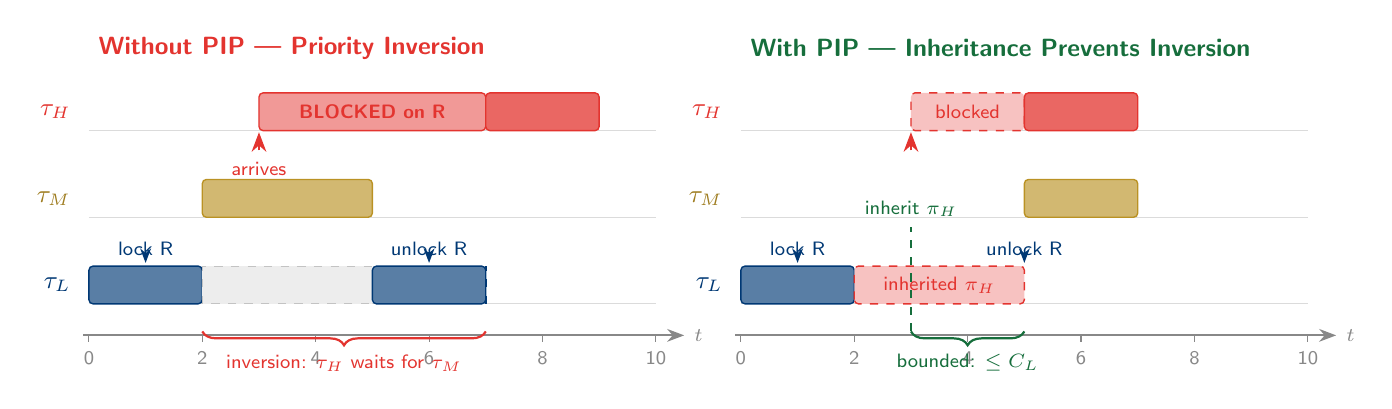
\begin{tikzpicture}[>=Stealth,font=\sffamily,x=0.72cm,y=1cm]

  \def\h{0.48}
  \def\rH{3.2}   % tau_H row base
  \def\rM{2.1}   % tau_M row base
  \def\rL{1.0}   % tau_L row base

  % ================================================================
  % LEFT PANEL — Priority Inversion (no fix)
  % Timeline [0,14]:
  %   tau_L: [0,2] runs, acquires R at t=1; [2,5] blocked by tau_M; [5,7] resumes; releases R at t=7
  %   tau_M: [2,5] preempts tau_L
  %   tau_H: [3,7] blocked waiting for R; [7,9] runs
  % ================================================================

  % panel label
  \node[rtred,font=\sffamily\small\bfseries,anchor=west] at (0,4.25)
        {Without PIP — Priority Inversion};

  % time axis
  \draw[axgray,line width=0.7pt,->] (-0.1,0.6) -- (10.5,0.6)
        node[right,font=\sffamily\scriptsize] {$t$};
  \foreach \t in {0,2,4,6,8,10}
    \draw[axgray] (\t,0.6) -- (\t,0.52)
          node[below,font=\sffamily\scriptsize,axgray] {\t};

  % row guides
  \foreach \y in {\rH,\rM,\rL}
    \draw[axgray!30,line width=0.4pt] (0,\y) -- (10,\y);

  % task labels
  \node[anchor=east,rtred,font=\sffamily\small\bfseries]
        at (-0.15,\rH+0.5*\h) {$\tau_H$};
  \node[anchor=east,kmgold!85!black,font=\sffamily\small\bfseries]
        at (-0.15,\rM+0.5*\h) {$\tau_M$};
  \node[anchor=east,kmblue,font=\sffamily\small\bfseries]
        at (-0.15,\rL+0.5*\h) {$\tau_L$};

  % tau_L: [0,2] runs (acquires R at t=1), [2,5] preempted, [5,7] runs, releases R
  \fill[kmblue!65,rounded corners=1.5pt] (0,\rL) rectangle (2,\rL+\h);
  \draw[kmblue,line width=0.5pt,rounded corners=1.5pt] (0,\rL) rectangle (2,\rL+\h);
  % preempted gap [2,5]
  \fill[axgray!15] (2,\rL) rectangle (5,\rL+\h);
  \draw[axgray!50,line width=0.4pt,dashed] (2,\rL) rectangle (5,\rL+\h);
  \fill[kmblue!65,rounded corners=1.5pt] (5,\rL) rectangle (7,\rL+\h);
  \draw[kmblue,line width=0.5pt,rounded corners=1.5pt] (5,\rL) rectangle (7,\rL+\h);

  % mutex R annotation on tau_L row
  \node[kmblue,font=\sffamily\scriptsize] at (1,\rL+\h+0.22) {lock R};
  \draw[kmblue,line width=0.5pt,->] (1,\rL+\h+0.18) -- (1,\rL+\h+0.04);
  \node[kmblue,font=\sffamily\scriptsize] at (6,\rL+\h+0.22) {unlock R};
  \draw[kmblue,line width=0.5pt,->] (6,\rL+\h+0.18) -- (6,\rL+\h+0.04);
  % unlock at t=7 end of block
  \draw[kmblue,line width=0.8pt,dashed] (7,\rL) -- (7,\rL+\h);

  % tau_M: [2,5]
  \fill[kmgold!65,rounded corners=1.5pt] (2,\rM) rectangle (5,\rM+\h);
  \draw[kmgold,line width=0.5pt,rounded corners=1.5pt] (2,\rM) rectangle (5,\rM+\h);

  % tau_H: [0,3] arrives and runs briefly, [3,7] BLOCKED on R (red), [7,9] runs
  \fill[rtred!50,rounded corners=1.5pt] (3,\rH) rectangle (7,\rH+\h);
  \draw[rtred,line width=0.5pt,rounded corners=1.5pt] (3,\rH) rectangle (7,\rH+\h);
  \node[rtred,font=\sffamily\scriptsize\bfseries] at (5,\rH+0.5*\h) {BLOCKED on R};
  \fill[rtred!75,rounded corners=1.5pt] (7,\rH) rectangle (9,\rH+\h);
  \draw[rtred,line width=0.5pt,rounded corners=1.5pt] (7,\rH) rectangle (9,\rH+\h);

  % tau_H arrival arrow
  \draw[rtred,line width=0.9pt,->] (3,\rH-0.25) -- (3,\rH-0.02);
  \node[rtred,font=\sffamily\scriptsize,below] at (3,\rH-0.28) {arrives};

  % Inversion brace
  \draw[rtred,line width=0.8pt,decorate,
        decoration={brace,amplitude=5pt,mirror}]
        (2,0.65) -- (7,0.65);
  \node[rtred,font=\sffamily\scriptsize] at (4.5,0.25)
        {inversion: $\tau_H$ waits for $\tau_M$};

  % ================================================================
  % RIGHT PANEL — With PIP (Priority Inheritance Protocol)
  % Timeline [0,14]:
  %   tau_L: [0,2], acquires R at 1; inherits H priority at t=3; [2,5] runs (not preempted by tau_M); releases R t=5
  %   tau_M: [5,7] runs (after tau_L releases R)
  %   tau_H: [3,5] blocked; [5,7] runs
  % ================================================================

  \def\xoff{11.5}  % horizontal offset for right panel

  % panel label
  \node[rtgreen!70!black,font=\sffamily\small\bfseries,anchor=west]
        at (\xoff,4.25) {With PIP — Inheritance Prevents Inversion};

  % time axis
  \draw[axgray,line width=0.7pt,->] (\xoff-0.1,0.6) -- (\xoff+10.5,0.6)
        node[right,font=\sffamily\scriptsize] {$t$};
  \foreach \t in {0,2,4,6,8,10}
    \draw[axgray] (\xoff+\t,0.6) -- (\xoff+\t,0.52)
          node[below,font=\sffamily\scriptsize,axgray] {\t};

  % row guides
  \foreach \y in {\rH,\rM,\rL}
    \draw[axgray!30,line width=0.4pt] (\xoff,\y) -- (\xoff+10,\y);

  % task labels
  \node[anchor=east,rtred,font=\sffamily\small\bfseries]
        at (\xoff-0.15,\rH+0.5*\h) {$\tau_H$};
  \node[anchor=east,kmgold!85!black,font=\sffamily\small\bfseries]
        at (\xoff-0.15,\rM+0.5*\h) {$\tau_M$};
  \node[anchor=east,kmblue,font=\sffamily\small\bfseries]
        at (\xoff-0.15,\rL+0.5*\h) {$\tau_L$};

  % tau_L: [0,2] runs (acquires R at 1); [2,5] runs with inherited priority (not preempted)
  \fill[kmblue!65,rounded corners=1.5pt]
        (\xoff,\rL) rectangle (\xoff+2,\rL+\h);
  \draw[kmblue,line width=0.5pt,rounded corners=1.5pt]
        (\xoff,\rL) rectangle (\xoff+2,\rL+\h);
  % inherited-priority section [2,5] — different shade
  \fill[rtred!30,rounded corners=1.5pt]
        (\xoff+2,\rL) rectangle (\xoff+5,\rL+\h);
  \draw[rtred,line width=0.5pt,rounded corners=1.5pt,dashed]
        (\xoff+2,\rL) rectangle (\xoff+5,\rL+\h);
  \node[rtred,font=\sffamily\scriptsize] at (\xoff+3.5,\rL+0.5*\h)
        {inherited $\pi_H$};
  % tau_L done after t=5
  % tau_M: [5,7]
  \fill[kmgold!65,rounded corners=1.5pt]
        (\xoff+5,\rM) rectangle (\xoff+7,\rM+\h);
  \draw[kmgold,line width=0.5pt,rounded corners=1.5pt]
        (\xoff+5,\rM) rectangle (\xoff+7,\rM+\h);

  % tau_H: [3,5] blocked (shorter, ends at 5), [5,7] runs
  \fill[rtred!30,rounded corners=1.5pt]
        (\xoff+3,\rH) rectangle (\xoff+5,\rH+\h);
  \draw[rtred,line width=0.5pt,rounded corners=1.5pt,dashed]
        (\xoff+3,\rH) rectangle (\xoff+5,\rH+\h);
  \node[rtred,font=\sffamily\scriptsize] at (\xoff+4,\rH+0.5*\h) {blocked};
  \fill[rtred!75,rounded corners=1.5pt]
        (\xoff+5,\rH) rectangle (\xoff+7,\rH+\h);
  \draw[rtred,line width=0.5pt,rounded corners=1.5pt]
        (\xoff+5,\rH) rectangle (\xoff+7,\rH+\h);

  % annotations
  \node[kmblue,font=\sffamily\scriptsize] at (\xoff+1,\rL+\h+0.22) {lock R};
  \draw[kmblue,line width=0.5pt,->] (\xoff+1,\rL+\h+0.18) -- (\xoff+1,\rL+\h+0.04);
  \node[kmblue,font=\sffamily\scriptsize] at (\xoff+5,\rL+\h+0.22) {unlock R};
  \draw[kmblue,line width=0.5pt,->] (\xoff+5,\rL+\h+0.18) -- (\xoff+5,\rL+\h+0.04);

  % tau_H arrives
  \draw[rtred,line width=0.9pt,->] (\xoff+3,\rH-0.25) -- (\xoff+3,\rH-0.02);

  % PIP annotation
  \draw[rtgreen!70!black,line width=0.7pt,dashed]
        (\xoff+3,0.65) -- (\xoff+3,\rL+\h+0.5);
  \node[rtgreen!70!black,font=\sffamily\scriptsize,above] at (\xoff+3,\rL+\h+0.5)
        {inherit $\pi_H$};

  % Bounded blocking brace
  \draw[rtgreen!70!black,line width=0.8pt,decorate,
        decoration={brace,amplitude=5pt,mirror}]
        (\xoff+3,0.65) -- (\xoff+5,0.65);
  \node[rtgreen!70!black,font=\sffamily\scriptsize] at (\xoff+4,0.25)
        {bounded: $\le C_L$};

\end{tikzpicture}
\end{document}
